\subsection{Matching}
Matching in an undirected graph $G=(V, E)$ is subset $M \subset E$ such that each vertex $v$ has at most one edge in $M$ touching it. In this way, we are pairing up vertices so each vertex can get paired to at most one of the vertex or to none of them.

Here is an example as follows:

\begin{figure}[H]
	\centering
	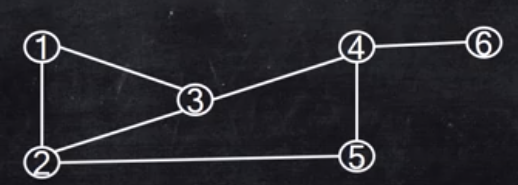
\includegraphics[width=0.5\textwidth]{fig/match.png}
\end{figure} 

In the example, $\{(1, 2), (4, 5)\}$ is a matching with 2 edges in it. $\{(1, 3), (2, 5), (4, 6)\}$ is another matching with 3 edges.

\subsection{Bipartite Graph}
Bipartite graphs are graphs $G = (V, E)$ where $V$ can be partitioned into $V_1$ and $V_2$ so that all edges go between $V_1$ and $V_2$.

Finding maximum matching in bipartite graphs is important.

\subsection{Solving Bipartite Matching via Flows}
In the following example, the left-hand-side is a bipartite graph. To solve bipartite problem by flows, first convert the graph into a flow network as the right hand side.
\begin{figure}[H]
	\centering
	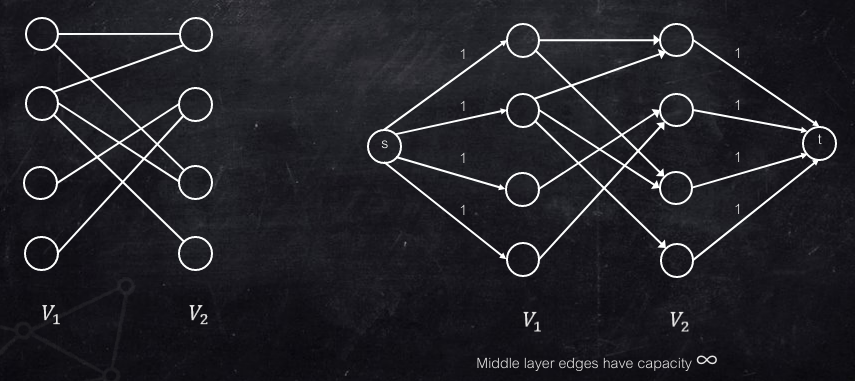
\includegraphics[width=0.5\textwidth]{fig/bipartition.png}
\end{figure} 
To solve the problem,
\begin{itemize}
	\item Find max flow in this network
	\item Recall that it will be integral
	\item Since the total capacity into each vertex in $v \in V_1$ is 1, at most one edge touching $v$ in middle layer (original bipartite graph) can carry flow out. That sounds like a matching!
	\item Similarly, since total capacity out of any vertex $v \in V_2$  is 1, at most one edge touching $w$ in middle layer can carry flow in.
	\item So, choose the matching to be all the edges in the middle layer that carry non-zero flow.
\end{itemize}

\subsection{Correctness}
\paragraph{Main Idea:} If bipartite graph has a matching of size $k$, then flow network has flow of value $k$. Conversely, if flow network has flow of value $\ell$, then there is a matching of size $\ell$. So, maximum matching corresponds to max flow value and it is what the max flow algorithm finds!

\subsubsection{Hall's theorem}
Max-flow min-cut theorem allows us to make an important observation about matching in bipartite graphs. Say a matching is perfect if it matches all vertices.

For a set of vertices $S$, define the neighborhood of $s$ as $\Gamma(S) = \{v: \exists u \in S: (u, v) \in E\}$.
\begin{theorem}
	A bipartite graph $G=(V_1 \cup V_2, E)$ has a perfect matching if and only if:
	\begin{itemize}
		\item $|V_1| = |V_2|$
		\item $\forall S \subseteq V_1, |\Gamma(S)| \ge |S|$
	\end{itemize}
\end{theorem}

\begin{proof}
	For a perfect matching to exist, the conditions of Hall's Theorem are clearly necessary. For the first condition, if the two sides have different numbers of vertices, no perfect matching can exist. For the second condition, if $|\Gamma(S)| < |S|$, vertices in $S$ cannot all be matched, which is shown in the following figure.
	\begin{figure}[H]
		\centering
		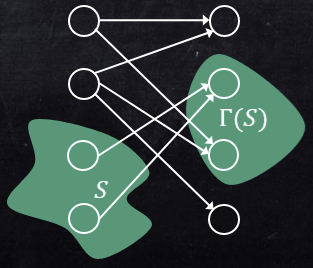
\includegraphics[width=0.3\textwidth]{fig/hall-theorem.png}
	\end{figure} 

	For the other direction, suppose for all sets $S \subseteq V_1$, $|\Gamma(S)| \ge |S|$ holds true. We will show by contradiction that the min-cut in the flow network for $G$ must have capacity $n = |V_1| = |V_2|$. Then by max-flow-min-cut theorem, the max flow will also be size of $n$. Finally, this implies that $n$ edges in middle layer are carrying flow, which means that the matching we get is of size $n$.
	
	Suppose for contradiction there is a min-cut of size less than $n$. Let's picture this situation,
	\begin{figure}[H]
	\centering
	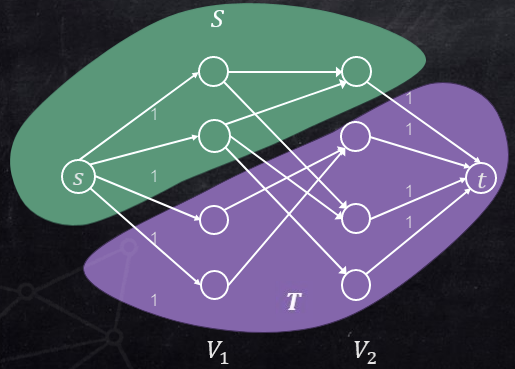
\includegraphics[width=0.3\textwidth]{fig/hall-theorem-proof.png}
	\end{figure} 	
	
	There are four sets in the graph, $S \cap V_1$, $S \cap V_2$, $T \cap V_1$, $T \cap V_2$. By observing, we get the facts that

	\begin{itemize}
		\item Edges from $s$ to $T \cap V_1$ cross the cut in forward direction with total capacity $|T \cap V_1|$.
		\item Edge from $S \cap V_2$ to $t$ cross the cut in forward direction with total capacity $|S \cap V_2|$.
		\item Other edges from $s$ and to $t$ do not cross the cut.
	\end{itemize}

	Note that none of the middle layer edges can cross the cut in the forward direction, because they have infinite capacity, and this would make the cut have infinite capacity. But a min cut will have finite capacity.
	
	Moreover, we do not care if they cross the cut in the backward direction, because such edges do not contribute to cut capacity.
	
	Therefore, the capacity of min cut = $|T \cap V_1| + |S \cap V_2|$.
	
	There are $n$ total vertices in $V_1$. They are either in $S$ or in $T$. So we can rewrite capacity as $(n- |S \cap V_1|) + |S \cap V_2|$. 
	
	Since the cut is of finite capacity, all neighbors of $S \cap V_1$ are in $S \cap V_2$. By hypothesis of hall's theorem, for any set in $V_1$, the size of its neighbor is at least as large as it is. So $|S \cap V_1| \le |S \cap V_2|$.
	
	Thus $(n- |S \cap V_1|) + |S \cap V_2| = n + (|S \cap V_2| - |S \cap V_1|) \ge n$.
	So the min cut is actually of size at least $n$, and so is the max flow value. This means the graph must have a perfect matching.
	
\end{proof}